% ============================================================
% 第5章：外积与行列式、张量运算（张量积、Kronecker积、张量缩约）、本章小结
% ============================================================

\section{外积与行列式}
\label{sec:ls-exterior-determinants}
\label{sec:linear-algebra-scalar-readouts}

内积回答一个向量有多长、两个向量夹角多大；把一组向量看成一个整体，还需要测量它们张成的平行多面体有多大。平行四边形的面积、平行六面体的体积都不是逐对长度相加能得到的量：它们由向量之间的相对方向共同决定，并且在两个向量交换位置时改变指向。本节先用一种满足交替性的多线性乘法建立外积，再在最高维得到行列式，说明它怎样测量体积缩放、怎样判断退化，以及怎样把特征值问题化为一个多项式方程。行列式只对每一列分别线性，与第~\ref{sec:ls-matrix-contractions}节对整个矩阵线性的迹是两种不同的标量读取。

\subsection{外积与有向体积}

\paragraph{外积（楔积）的定义}

内积把两个向量合成一个标量，面积和体积却要求把$k$个向量合成一个仍带有$k$个槽位的量：交换其中两个输入，结果应当改变指向而不是消失。设$V=\mathbb R^d$，对$k$个向量$\bm v_1,\ldots,\bm v_k$定义它们的\term{外积}（exterior product，又称\term{楔积}wedge product）$\bm v_1\wedge\cdots\wedge\bm v_k$，要求它满足两条规则。

第一是多线性：对每个因子分别保持线性，即把某个$\bm v_i$换成$a\bm u+b\bm w$时，整个楔积等于$a(\cdots\wedge\bm u\wedge\cdots)+b(\cdots\wedge\bm w\wedge\cdots)$，其余因子不动。第二是交替性：交换相邻两个因子，楔积变号，
\[
 \cdots\wedge\bm v_i\wedge\bm v_j\wedge\cdots
 =-\cdots\wedge\bm v_j\wedge\bm v_i\wedge\cdots.
\]
由交替性立刻得到，两个因子相同的楔积为零：交换两个相同因子，楔积等于自身的相反数，只能为零。由此还可推出，任一因子是其余因子的线性组合时，整个楔积为零：代入后展开式中每一项都含有重复因子。

取标准基$\bm e_1,\ldots,\bm e_d$后，每个楔积都能用基楔积展开。下标满足$i_1<\cdots<i_k$的基楔积$\bm e_{i_1}\wedge\cdots\wedge\bm e_{i_k}$共有$\binom{d}{k}$个，它们构成$k$阶楔积空间的一组基；任意$\bm v_j=\sum_i v_{j,i}\bm e_i$代入并展开，只保留下标互不相同的项，再按交替性把下标排成递增次序。当$k>d$时取不出$k$个互不相同的下标，故$k>d$的楔积恒为零。

二阶楔积$\bm u\wedge\bm v$记录由$\bm u,\bm v$张成的平行四边形：它的绝对值是面积，符号是定向。在$\mathbb R^2$中，
\[
 \bm u\wedge\bm v
 =(u_1\bm e_1+u_2\bm e_2)\wedge(v_1\bm e_1+v_2\bm e_2)
 =(u_1v_2-u_2v_1)\,\bm e_1\wedge\bm e_2,
\]
其中$\bm e_1\wedge\bm e_1$与$\bm e_2\wedge\bm e_2$为零，$\bm e_2\wedge\bm e_1=-\bm e_1\wedge\bm e_2$。系数$u_1v_2-u_2v_1$正是平行四边形的有向面积。例如$\bm u=(1,0)^\top$、$\bm v=(1,1)^\top$给出$1$；交换两向量得$-1$，面积不变而定向翻转。三个向量的楔积$\bm u\wedge\bm v\wedge\bm w$在$\mathbb R^3$中的系数，绝对值就是平行六面体的体积，带符号时称为\term{有向体积}。

交替性还直接给出退化判据：$k\leq d$时，$\bm v_1,\ldots,\bm v_k$线性相关当且仅当楔积为零。相关时楔积为零已如上述；无关时这组向量可以扩充为一组基，其楔积与相应基楔积只差一个非零系数。楔积为零，等价于这组向量张成的平行多面体被压低了维数。例如$\bm u=(1,1)^\top$、$\bm v=(2,2)^\top$给出$2-2=0$，平行四边形退化成一条线段。

交换两个因子只改变符号、不改变绝对值，这正是“定向”的代数表达。对一般排列$\pi$，
\[
 \bm v_{\pi(1)}\wedge\cdots\wedge\bm v_{\pi(k)}
 =\operatorname{sgn}(\pi)\,\bm v_1\wedge\cdots\wedge\bm v_k,
\]
其中$\operatorname{sgn}(\pi)=(-1)^{N(\pi)}$，$N(\pi)$为逆序对数，即满足$i<j$而$\pi(i)>\pi(j)$的索引对数；每做一次相邻交换，$N(\pi)$改变$1$，符号翻转一次。

\subsection{行列式的定义与性质}
\label{sec:ls-determinant-properties}
\label{sec:prelim-determinants}

在$d$维空间中取$d$个向量，最高维楔积只有一个基元素$\bm e_1\wedge\cdots\wedge\bm e_d$。把线性作用$\bm A$依次作用到标准基上，
\[
 \bm A\bm e_1\wedge\cdots\wedge\bm A\bm e_d
 =(\det\bm A)\,\bm e_1\wedge\cdots\wedge\bm e_d,
\]
标量$\det\bm A$就是\term{行列式}（determinant）：它是作用$\bm A$把单位立方体变成平行多面体时的有向体积倍数，绝对值为体积比，符号表示定向是否翻转。图~\ref{fig:ls-determinant-oriented-volume} 在平面上画出这一缩放。
\begin{figure*}[htbp]
  \centering
  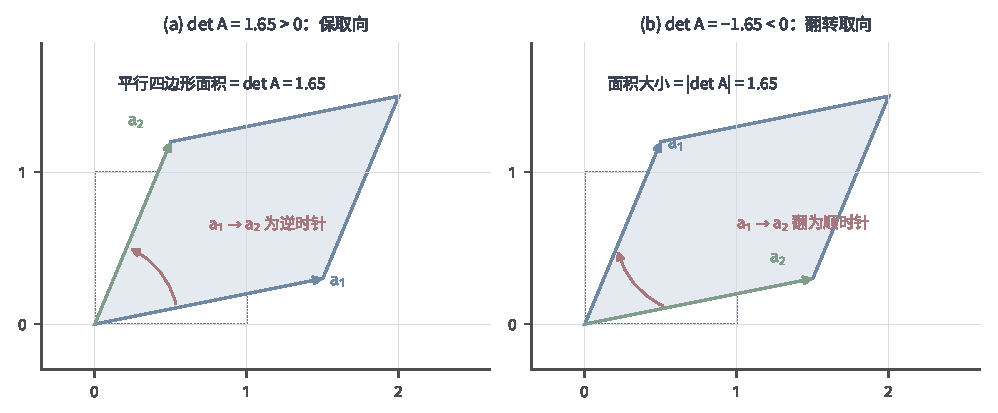
\includegraphics[width=169mm]{figures/01-mathematical-preliminaries-upper/02-linear-spaces/matplotlib/ls-determinant-oriented-volume/ls-determinant-oriented-volume.pdf}
  \caption{行列式作为有向体积的缩放。左：单位正方形由$\bm e_1=(1,0)$、$\bm e_2=(0,1)$张成，面积为$1$。中：$\bm A=\bigl(\begin{smallmatrix}2&0.5\\0&1.5\end{smallmatrix}\bigr)$把它映成由$\bm A\bm e_1=(2,0)$、$\bm A\bm e_2=(0.5,1.5)$张成的平行四边形，有向面积为$2\cdot1.5-0.5\cdot0=3=\det\bm A>0$（保定向）。右：$\bm A$把$\bm e_1$反射到$(-2,0)$，有向面积为$-3$（反定向）。向量与数值均为解析教学例。}
  \label{fig:ls-determinant-oriented-volume}
\end{figure*}

为了直接由矩阵元素计算，把$\bm A\bm e_j=\sum_i a_{i,j}\bm e_i$代入楔积展开，得到有限和
\[
 \det\bm A
 =\sum_{\pi\in S_d}\operatorname{sgn}(\pi)
   \prod_{i=1}^d a_{i,\pi(i)}.
\]
这里$S_d$是$\{1,\ldots,d\}$到自身的全部双射，每个$\pi$规定第$i$行选取第$\pi(i)$列。$d=2$时两种列次序的逆序对数分别为$0$与$1$，正好得到$ad-bc$。行列式因而是矩阵元素的多项式。例如$\begin{pmatrix}1&2\\3&4\end{pmatrix}$的行列式为$-2$，与它的迹$5$是两个不同的量。

由楔积的规则可逐条读出行列式的列变换性质：对每一列分别线性；交换两列变号，两列相同则为零；把某列的倍数加到另一列上不改变行列式。把排列展开中的$\pi$换成逆排列，得到$\det(\bm A^\top)=\det\bm A$，所以这些规则对行同样成立。三角矩阵的排列展开中只有主对角线一项非零，故三角行列式等于对角元之积，$\det\bm I_d=1$。行列式不是对整个矩阵线性的函数：$d\geq2$时一般$\det(\bm A+\bm B)\neq\det\bm A+\det\bm B$。

\paragraph{行列式乘法性与可逆判据}

复合两次作用时，体积缩放倍数应当相乘。由楔积的多线性，
\[
 (\bm A\bm B)\bm e_1\wedge\cdots\wedge(\bm A\bm B)\bm e_d
 =(\det\bm B)\,\bm A\bm e_1\wedge\cdots\wedge\bm A\bm e_d
 =(\det\bm A)(\det\bm B)\,\bm e_1\wedge\cdots\wedge\bm e_d,
\]
其中第一步把$\bm B\bm e_j=\sum_i b_{i,j}\bm e_i$代入后，$\bm A$作用在展开式的各项上，系数正是$\det\bm B$。于是
\[
 \det(\bm A\bm B)=\det\bm A\,\det\bm B.
\]
列线性相关时楔积为零，行列式为零；列线性无关时楔积非零，行列式非零。所以方阵可逆恰好等价于行列式非零，且可逆时$\det(\bm A^{-1})=1/\det\bm A$。

在第~\ref{sec:ls-matrix-equivalences}节的相似关系$\bm B=\bm P^{-1}\bm A\bm P$中，由乘法性
\[
 \det\bm B
 =\det(\bm P^{-1})\det\bm A\det\bm P
 =\det\bm A,
\]
相似变换不改变行列式；它与第~\ref{sec:ls-matrix-contractions}节迹的相似不变性一起，是判断两个矩阵能否记录同一映射时可直接计算的两个标量不变量。双线性型在两个输入同时换基时按合同$\bm B=\bm P^\top\bm A\bm P$变换，此时$\det\bm B=(\det\bm P)^2\det\bm A$：合同只保持行列式的符号与非零性，不保持数值。

\paragraph{特征多项式}

行列式把第~\ref{sec:ls-matrix-powers}节的特征值问题化为一个标量方程。$\lambda$是$\bm A$的特征值，当且仅当$(\bm A-\lambda\bm I)\bm v=\bm0$有非零解，即$\bm A-\lambda\bm I$不可逆，也即$\det(\lambda\bm I-\bm A)=0$。定义
\begin{equation}
 p_{\bm A}(z)=\det(z\bm I-\bm A),
 \label{eq:matrix-analysis-characteristic-polynomial}
\end{equation}
称为\term{特征多项式}（characteristic polynomial）。排列展开中只有对角线一项含$z^d$，故它是首项系数为$1$的$d$次实多项式，实特征值恰为它的实根。以$\bm A=\begin{pmatrix}0.8&4\\0&0.5\end{pmatrix}$为例，$p_{\bm A}(z)=(z-0.8)(z-0.5)$，与第~\ref{sec:ls-matrix-powers}节找到的两条特征方向相符；$90^\circ$旋转的特征多项式$z^2+1$没有实根，因而没有实特征向量。相似矩阵的特征多项式相同：$\det(z\bm I-\bm P^{-1}\bm A\bm P)=\det\bigl(\bm P^{-1}(z\bm I-\bm A)\bm P\bigr)=p_{\bm A}(z)$。

根$\lambda$在$p_{\bm A}$中的重数称为\term{代数重数}，特征空间的维数$\dim\ker(\bm A-\lambda\bm I)$称为\term{几何重数}。把$\lambda$的特征空间的一组基（设有$g$个向量）扩充成全空间的基，$\bm A$在新基下成为分块上三角$\begin{pmatrix}\lambda\bm I_g&*\\\bm0&\bm C\end{pmatrix}$，特征多项式含因子$(z-\lambda)^g$，故几何重数不超过代数重数。例如$\begin{pmatrix}0.8&1\\0&0.8\end{pmatrix}$的特征多项式为$(z-0.8)^2$，代数重数为$2$，几何重数却只有$1$。

不同特征值的特征空间之和是直和：若$\sum_\lambda\bm w_\lambda=\bm0$且$\bm w_\lambda$属于相应特征空间，其中非零的$\bm w_\lambda$是不同特征值的特征向量，由第~\ref{sec:ls-matrix-powers}节它们线性无关，所以每个$\bm w_\lambda=\bm0$。因此各特征空间的基合在一起仍线性无关。由此得到可对角化的判据：$\bm A$实可对角化，当且仅当$p_{\bm A}$能分解为实一次因子之积，且每个特征值的几何重数等于代数重数。充分性是因为此时几何重数之和等于$d$，各特征空间的基合成一组特征基；必要性是因为$\bm A=\bm V\bm\Lambda\bm V^{-1}$时$p_{\bm A}(z)=\prod_i(z-\lambda_i)$，$\lambda$在$\bm\Lambda$对角线上出现的次数既是代数重数，也是$\bm\Lambda-\lambda\bm I$的零空间维数，而相似变换不改变零空间维数。

\paragraph{余子式与古典伴随恒等式}

行列式还可以按一行展开。对$d\geq2$，删除第$i$行、第$j$列得到的$(d-1)$阶子矩阵记为$\bm A^{(i,j)}$，定义\term{代数余子式}（cofactor）
\[
 C_{i,j}=(-1)^{i+j}\det\bm A^{(i,j)}.
\]
把排列展开按第$i$行选取的列分类，得到$\det\bm A=\sum_{j=1}^d a_{i,j}C_{i,j}$；按列同样有$\det\bm A=\sum_{i=1}^d a_{i,j}C_{i,j}$。把全部代数余子式排成矩阵$\bm C$，其转置称为\term{古典伴随}（classical adjugate）$\operatorname{adj}(\bm A)=\bm C^\top$。

\begin{theorem}[古典伴随恒等式]
\label{thm:ls-adjugate-identity}
对任意$d$阶方阵$\bm A$，
\[
 \bm A\,\operatorname{adj}(\bm A)
 =\operatorname{adj}(\bm A)\,\bm A
 =(\det\bm A)\,\bm I_d.
\]
\end{theorem}
\begin{proof}
乘积$\bm A\bm C^\top$的$(i,k)$元素为$\sum_j a_{i,j}C_{k,j}$。当$i=k$时，这正是沿第$i$行展开的$\det\bm A$；当$i\neq k$时，它是把第$k$行换成第$i$行后的矩阵沿第$k$行的展开，新矩阵有两行相同，行列式为零。于是$\bm A\bm C^\top=(\det\bm A)\bm I_d$。按列展开同样得到$\bm C^\top\bm A=(\det\bm A)\bm I_d$。
\end{proof}

古典伴随是由余子式得到的代数构造，与第~\ref{sec:ls-adjoints}节由内积配对定义的伴随不是同一个对象。$\det\bm A\neq0$时，恒等式给出逆的代数表达$\bm A^{-1}=\operatorname{adj}(\bm A)/\det\bm A$，二阶时即$\begin{pmatrix}a&b\\c&d\end{pmatrix}^{-1}=\frac1{ad-bc}\begin{pmatrix}d&-b\\-c&a\end{pmatrix}$。高阶时展开余子式的代价是阶乘级的，恒等式主要作为证明工具，例如第~\ref{sec:ls-matrix-power-behavior}节的Cayley--Hamilton定理。

\section{张量运算}
\label{sec:ls-tensor-operations}

前面的运算大多把同类对象合成同类对象。张量运算处理多个槽位：张量积把多个输入的槽位全部保留下来，组合成一个带更多轴的对象；Kronecker积是两个矩阵的张量积在坐标下的分块记录；缩约则反过来，指定一对槽位对齐求和，把多轴对象汇总成更低阶的对象。三者共同组成多轴数据的基本运算，内积、矩阵乘法与迹都是其中的特例。

\subsection{张量积}
\label{sec:ls-tensor-products}
\label{sec:linear-algebra-joint-operations}

\subsubsection{定义与含义}

\paragraph{张量积与简单张量}

设$\bm x\in\mathbb R^m$、$\bm y\in\mathbb R^n$，它们的\term{张量积}（tensor product）$\bm x\otimes\bm y$是一个$m\times n$数组，元素为$(\bm x\otimes\bm y)_{i,j}=x_i y_j$。这样的对象称为\term{简单张量}（simple tensor）。例如$\bm x=(1,2)^\top$、$\bm y=(3,-1)^\top$给出$\bm x\otimes\bm y=\begin{pmatrix}3&-1\\6&-2\end{pmatrix}$，每一行都是$\bm y$的倍数，每一列都是$\bm x$的倍数。一般张量是若干简单张量之和$\sum_s\bm x_s\otimes\bm y_s$；并非每个二阶张量都能写成单个简单张量，正如并非每个矩阵都是秩一矩阵。图~\ref{fig:ls-tensor-product-slots} 展示张量积怎样保留两个因子的槽位。
\begin{figure}[htbp]
  \centering
  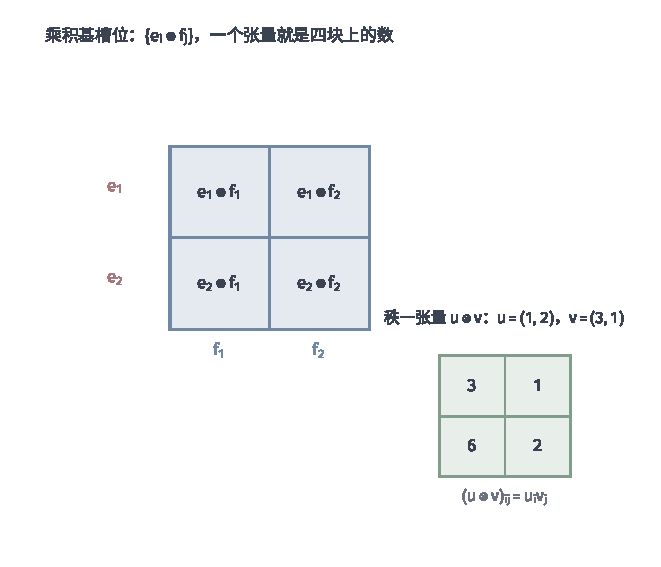
\includegraphics[width=112mm]{figures/01-mathematical-preliminaries-upper/02-linear-spaces/matplotlib/ls-tensor-product-slots/ls-tensor-product-slots.pdf}
  \caption{张量积并排保留两个因子的槽位。左：$\bm u\in\mathbb R^2$、$\bm v\in\mathbb R^3$。右：$\bm u\otimes\bm v$排成$2\times3$网格，每行由$\bm v$方向复制并按$u_i$缩放；它是秩一张量，数值由$\bm u=(1,0.6)$、$\bm v=(1,0.5,0.2)$直接相乘得到，是教学构造。}
  \label{fig:ls-tensor-product-slots}
\end{figure}

取$\mathbb R^m$的基$\bm e_i$与$\mathbb R^n$的基$\bm f_j$，产品基$\bm e_i\otimes\bm f_j$共$mn$个，构成张量积空间的一组基，故维数为$mn$。三个向量的张量积$(\bm x\otimes\bm y\otimes\bm z)_{i,j,k}=x_i y_j z_k$保留三条轴，多重张量积按同样规则逐槽位相乘。

张量积的作用是把双线性映射变成线性映射。给定双线性映射$B:\mathbb R^m\times\mathbb R^n\to W$，存在唯一的线性映射$\widetilde B:\mathbb R^m\otimes\mathbb R^n\to W$使$\widetilde B(\bm x\otimes\bm y)=B(\bm x,\bm y)$：先在产品基上规定$\widetilde B(\bm e_i\otimes\bm f_j)=B(\bm e_i,\bm f_j)$，再线性延拓即可。以欧氏内积$B(\bm x,\bm y)=\bm x^\top\bm y$为例，提升后的线性映射把$\bm x\otimes\bm y$送到$\sum_ix_iy_i$，也就是对数组$\bm x\otimes\bm y$的对角线求和——这正是后面的缩约。

二阶张量与矩阵是同一组数的两种记录：张量强调槽位来自哪一组输入，矩阵强调行列在复合中的角色。二者由第~\ref{sec:ls-reshaping}节的重排互相转换，数值不变。

\subsubsection{运算性质}

张量积对两个因子分别线性：$(a\bm x)\otimes\bm y=\bm x\otimes(a\bm y)=a(\bm x\otimes\bm y)$，且对加法分配；括号可以在槽位间移动，$(\bm x\otimes\bm y)\otimes\bm z=\bm x\otimes(\bm y\otimes\bm z)$。交换两个槽位对应轴置换：$\bm x\otimes\bm y$的$(i,j)$元素$x_iy_j$是$\bm y\otimes\bm x$的$(j,i)$元素，两者互为转置。

第~\ref{sec:ls-exterior-determinants}节的楔积可以由张量积经反对称化得到：$\bm x\wedge\bm y$对应$\bm x\otimes\bm y-\bm y\otimes\bm x$。这里只指出联系，楔积的构造不依赖张量积。

在Frobenius内积下，简单张量的配对与范数都分离：
\[
 \langle\bm x\otimes\bm y,\bm x'\otimes\bm y'\rangle_{\mathrm F}
 =\langle\bm x,\bm x'\rangle\langle\bm y,\bm y'\rangle,
 \qquad
 \lVert\bm x\otimes\bm y\rVert_{\mathrm F}=\lVert\bm x\rVert\,\lVert\bm y\rVert,
\]
因为$\sum_{i,j}x_iy_jx'_iy'_j=(\sum_ix_ix'_i)(\sum_jy_jy'_j)$。以$\bm x=(1,2)^\top$、$\bm y=(3,-1)^\top$为例，乘积范数为$\sqrt5\cdot\sqrt{10}=5\sqrt2$，与直接对$\begin{pmatrix}3&-1\\6&-2\end{pmatrix}$求Frobenius范数一致。

\paragraph{Schur乘积定理}

配对的分离性给出一个关于逐项乘积的结论。设$\bm A,\bm B$均为半正定矩阵，由定理~\ref{thm:ls-gram-factor}，它们各有Gram因子$\bm A=\bm U^\top\bm U$、$\bm B=\bm V^\top\bm V$，即$A_{i,k}=\langle\bm u_i,\bm u_k\rangle$、$B_{i,k}=\langle\bm v_i,\bm v_k\rangle$，其中$\bm u_i,\bm v_i$是两个因子的列。考虑向量组$\{\bm u_i\otimes\bm v_i\}$，其Gram矩阵为
\[
 \langle\bm u_i\otimes\bm v_i,\bm u_k\otimes\bm v_k\rangle_{\mathrm F}
 =\langle\bm u_i,\bm u_k\rangle\langle\bm v_i,\bm v_k\rangle
 =A_{i,k}B_{i,k}.
\]
Gram矩阵恒半正定，故逐项乘积$\bm A\odot\bm B$半正定，这就是\term{Schur乘积}定理。例如$\bm A=\bm B=\begin{pmatrix}1&1\\1&2\end{pmatrix}$，逐项乘积$\begin{pmatrix}1&1\\1&4\end{pmatrix}$的行列式为$3>0$、对角元为正，仍半正定。核方法中两个核矩阵的逐项乘积仍是合法核矩阵，依据就是这一定理。

\subsection{Kronecker积}
\label{sec:ls-kronecker-products}

当两个因子本身都是矩阵时，张量积空间上的联合作用可以写成一张分块矩阵，这就是Kronecker积。

\subsubsection{定义与含义}

\paragraph{Kronecker积的定义}

对$\bm A\in\mathbb R^{m\times n}$、$\bm B\in\mathbb R^{p\times q}$，定义
\begin{equation}
 \bm A\otimes\bm B
 =\begin{bmatrix}
  A_{1,1}\bm B&\cdots&A_{1,n}\bm B\\
  \vdots&\ddots&\vdots\\
  A_{m,1}\bm B&\cdots&A_{m,n}\bm B
 \end{bmatrix}\in\mathbb R^{mp\times nq}.
 \label{eq:linear-algebra-kronecker-product}
\end{equation}
每个块$A_{i,j}\bm B$是$\bm B$整体乘以$A_{i,j}$。图~\ref{fig:ls-kronecker-block-structure} 展示这种逐元素替换的分块结构。
\begin{figure}[htbp]
  \centering
  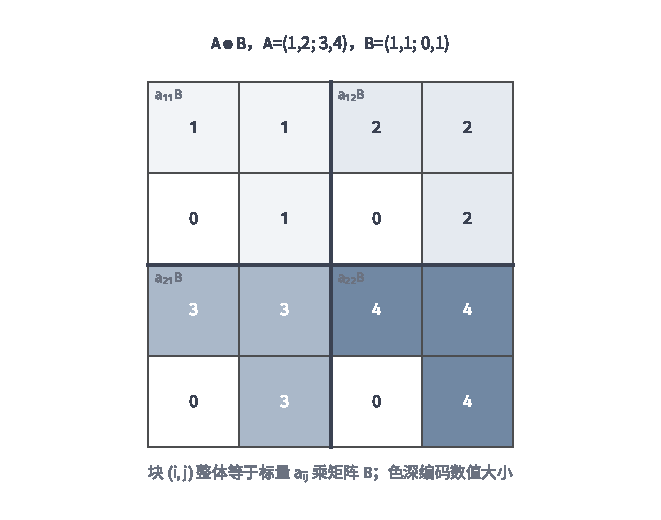
\includegraphics[width=112mm]{figures/01-mathematical-preliminaries-upper/02-linear-spaces/matplotlib/ls-kronecker-block-structure/ls-kronecker-block-structure.pdf}
  \caption{Kronecker积的分块结构。上：$\bm A=\bigl(\begin{smallmatrix}1&2\\3&4\end{smallmatrix}\bigr)$、$\bm B=\bigl(\begin{smallmatrix}10&20\\30&40\end{smallmatrix}\bigr)$。下：$\bm A\otimes\bm B$是把$\bm A$的每个元素替换为该元素乘$\bm B$得到的$4\times4$分块矩阵，块边界用白线强调。数值由定义直接计算，是教学例。}
  \label{fig:ls-kronecker-block-structure}
\end{figure}

在产品基$\bm e_i\otimes\bm f_j$下，$(\bm A\otimes\bm B)(\bm x\otimes\bm y)=(\bm A\bm x)\otimes(\bm B\bm y)$：第一个槽位只经过$\bm A$，第二个槽位只经过$\bm B$，两个作用并行而不串联。这与矩阵乘法把前后两次作用串成一条链形成对照。向量的张量积是它的特例：两个列向量的Kronecker积就是按行展开的$\bm x\otimes\bm y$。

\subsubsection{运算性质}

按成对索引分别求和，相容乘积满足混合乘积规则
\begin{equation}
 (\bm A\otimes\bm B)(\bm C\otimes\bm D)
 =(\bm A\bm C)\otimes(\bm B\bm D),
 \label{eq:matrix-analysis-kronecker-mixed-product}
\end{equation}
其中$\bm A\bm C$与$\bm B\bm D$分别相容：左侧的块$(i,k)$为$\sum_jA_{i,j}C_{j,k}\bm B\bm D$，恰是右侧的块。由此得到$(\bm A\otimes\bm B)^\top=\bm A^\top\otimes\bm B^\top$；两因子都可逆时$(\bm A\otimes\bm B)^{-1}=\bm A^{-1}\otimes\bm B^{-1}$；方阵情形下$\operatorname{tr}(\bm A\otimes\bm B)=\operatorname{tr}\bm A\operatorname{tr}\bm B$。

结合第~\ref{sec:ls-reshaping}节的向量化，对$\bm A\in\mathbb R^{p\times m}$、$\bm X\in\mathbb R^{m\times n}$、$\bm B\in\mathbb R^{n\times q}$，
\begin{equation}
 \operatorname{vec}(\bm A\bm X\bm B)
 =(\bm B^\top\otimes\bm A)\operatorname{vec}(\bm X).
 \label{eq:matrix-analysis-vec-kronecker}
\end{equation}
证明只需比较输出元素：两侧的$(i,j)$元素均为$\sum_{\ell=1}^m\sum_{k=1}^n A_{i,\ell}X_{\ell,k}B_{k,j}$。固定$\bm A,\bm B$后这是关于$\bm X$的线性映射，把两侧同时作用于未知矩阵的方程化成普通线性方程组。

表~\ref{tab:linear-algebra-products-and-shapes}汇总本章几种“乘法”的形状条件与索引作用。

\begin{table*}[htbp]
 \centering\small
 \begin{tabularx}{\linewidth}{@{}lXX@{}}
  \toprule
  运算 & 形状条件与输出 & 索引作用\\
  \midrule
  $\bm A\bm B$ & $(m\times n)(n\times p)\to m\times p$ & 汇总共同索引\\
  $\bm A\odot\bm B$ & 同为$m\times n$，输出仍为$m\times n$ & 同位置相乘，不求和\\
  $\bm A\otimes\bm B$ & $(m\times n)$与$(p\times q)\to(mp)\times(nq)$ & 保留两组成对索引\\
  $\langle\bm x,\bm y\rangle$ & 两个$n$维向量，输出标量 & 配对后汇总\\
  \bottomrule
 \end{tabularx}
 \caption{相乘符号对应不同操作。先检查消去哪些索引，再判断其线性性和输出含义。}
 \label{tab:linear-algebra-products-and-shapes}
\end{table*}

\subsection{张量缩约}
\label{sec:ls-tensor-contraction}

张量积把槽位全部保留，缩约则指定一对相容槽位，对齐相乘后求和，消去这对轴。

\subsubsection{定义与性质}

\paragraph{张量缩约的定义}

缩约须先指定参与求和的轴，并保证对应尺寸相同。例如$\bm A\in\mathbb R^{m\times d\times r}$、$\bm B\in\mathbb R^{d\times n\times r}$可定义
\[
 c_{i,j}=\sum_{k=1}^d\sum_{s=1}^r a_{i,k,s}b_{k,j,s},
\]
同时消去$k$与$s$两对轴。被求和的轴消失，其余轴保留：上例输出为$m\times n$矩阵。矩阵乘法是只消去一对轴的特例，内积是两个向量唯一一对轴的缩约。对$\bm X\in\mathbb R^{b\times\ell\times d}$的最后一轴作用$\bm W\in\mathbb R^{d\times h}$，$z_{i,j,r}=\sum_k x_{i,j,k}w_{k,r}$，输出形状为$b\times\ell\times h$。写出索引就能检查哪些轴被消去、哪些轴应当保留。图~\ref{fig:ls-tensor-contraction} 沿一对选中的轴求和并保留其余轴。
\begin{figure}[htbp]
  \centering
  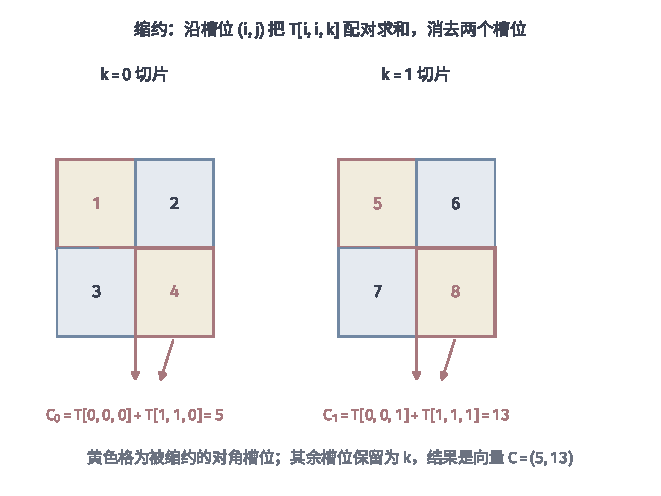
\includegraphics[width=112mm]{figures/01-mathematical-preliminaries-upper/02-linear-spaces/matplotlib/ls-tensor-contraction/ls-tensor-contraction.pdf}
  \caption{张量缩约沿选中的一对轴求和、保留其余轴。左：二阶张量按行和列着色；选中列轴（虚线箭头）沿列求和，输出对每行汇总为一个值。右：缩约后得到$3$个输出，分别对应原矩阵三行的行和，颜色由红(小)经黄到蓝(大)。张量与数值均为解析教学例。}
  \label{fig:ls-tensor-contraction}
\end{figure}

系数是简单张量时，缩约可以分开计算。一次读取同时依赖三组向量$\bm x\in\mathbb R^m$、$\bm y\in\mathbb R^n$、$\bm z\in\mathbb R^p$时，若系数数组是秩一张量$\bm a\otimes\bm b\otimes\bm c$，则
\begin{equation}
 \left\langle\bm a\otimes\bm b\otimes\bm c,
 \bm x\otimes\bm y\otimes\bm z\right\rangle_{\mathrm F}
 =(\bm a^\top\bm x)(\bm b^\top\bm y)(\bm c^\top\bm z),
 \label{eq:linear-algebra-rank-one-contraction}
\end{equation}
三重求和分离成三个内积的乘积。例如取$\bm a=(1,2)^\top$、$\bm b=(3,-1)^\top$、$\bm c=(2,1)^\top$，$\bm x=(2,1)^\top$、$\bm y=(1,1)^\top$、$\bm z=(1,-1)^\top$，三个内积依次为$4,2,1$，读取等于$8$。

固定配对对象后，缩约对被作用张量线性。多对轴的缩约是有限和，求和次序可以交换，结果与先消哪一对轴无关。$\operatorname{softmax}$、逐元素非线性等操作不属于缩约：一个模型即使由缩约和这些操作交替组成，固定系数时的线性也不代表整体线性。

\subsubsection{矩阵上的缩约}
\label{sec:ls-matrix-contractions}
\label{sec:prelim-matrix-trace}

\paragraph{迹的定义}

方阵最自然的缩约是把行轴与列轴对齐到同一索引后求和。对$n$阶方阵，定义\term{迹}（trace）
\[
 \operatorname{tr}(\bm A)=\sum_{i=1}^n A_{i,i}.
\]
例如$\bm A=\begin{pmatrix}1&2\\3&4\end{pmatrix}$的迹为$1+4=5$。迹是对角元之和，不是全部元素之和。有限和的线性规则直接给出$\operatorname{tr}(a\bm A+b\bm B)=a\operatorname{tr}(\bm A)+b\operatorname{tr}(\bm B)$。

矩阵乘法没有交换律，但乘积的迹在合法的循环移位下不变。对$\bm A\in\mathbb R^{m\times n}$、$\bm B\in\mathbb R^{n\times m}$，有限和换序给出
\begin{equation}
 \operatorname{tr}(\bm A\bm B)
 =\sum_{i=1}^m\sum_{j=1}^n A_{i,j}B_{j,i}
 =\operatorname{tr}(\bm B\bm A).
 \label{eq:linear-algebra-trace-cyclic}
\end{equation}
两个乘积甚至可以是不同阶的方阵；相等的是迹，不是矩阵本身。三因子只能循环移动，$\operatorname{tr}(\bm A\bm B\bm C)=\operatorname{tr}(\bm B\bm C\bm A)=\operatorname{tr}(\bm C\bm A\bm B)$，不能任意交换相邻因子：取$\bm A=\begin{pmatrix}1&0\\0&0\end{pmatrix}$、$\bm B=\begin{pmatrix}0&0\\1&0\end{pmatrix}$、$\bm C=\begin{pmatrix}0&1\\0&0\end{pmatrix}$，则$\bm A\bm B\bm C=\bm0$，而$\bm A\bm C\bm B=\begin{pmatrix}1&0\\0&0\end{pmatrix}$，迹分别为$0$与$1$。由循环性，相似变换不改变迹：
\[
 \operatorname{tr}(\bm P^{-1}\bm A\bm P)
 =\operatorname{tr}(\bm A\bm P\bm P^{-1})
 =\operatorname{tr}\bm A.
\]
迹与行列式一样，是第~\ref{sec:ls-matrix-equivalences}节相似关系下的标量不变量。

第~\ref{sec:ls-inner-products}节定义的Frobenius内积把对应位置相乘后相加，写成缩约就是
\[
 \langle\bm A,\bm B\rangle_{\mathrm F}
 =\sum_{i,j}A_{i,j}B_{i,j}
 =\operatorname{tr}(\bm A^\top\bm B),
\]
因为$\bm A^\top\bm B$第$j$个对角元为$\sum_i A_{i,j}B_{i,j}$，再对$j$求和恰好遍历所有位置。计算$\operatorname{tr}(\bm A\bm B)$时也不必形成乘积：只需$\sum_{i,j}A_{i,j}B_{j,i}$，代价为$mn$而非$m^2n$。

\section{本章小结}
\label{sec:ls-operations-summary}

本章回答第~\ref{chap:linear-representation}章记录下来的对象怎样运算。对每种运算，我们都规定了输入的相容条件与输出形状，说明了它的运算逻辑，并给出可以直接使用的性质。

第一组运算把对象合并成同类对象。加法与数乘要求形状一致，线性组合把多个记录合成一个，映射的叠加对应矩阵的逐项相加。“乘法”有两种含义：逐项乘法在同一位置相乘、不汇总任何索引，依赖坐标；矩阵乘法来自映射复合，汇总共同索引，满足结合律而不满足交换律。分块后块可以像数一样相乘。同一方阵的反复作用得到矩阵幂；特征方向是幂在其上只作标量缩放的方向，可对角化时幂化为对角元的乘方。转置、轴置换、reshape与向量化只改变记录位置，不改变数值，但会改变秩与诱导范数这类依赖排列的量。

第二组运算给对象以几何。内积把两个对象配成标量，由Cauchy--Schwarz不等式得到夹角；加权内积由正定矩阵给出，Gram因子定理说明它只是换了一组欧氏坐标；Gram矩阵记录一组向量的全部配对，非奇异当且仅当它们线性无关，由此得到正交直和。范数给出误差的大小：$\ell_p$范数由Hölder不等式联系，诱导矩阵范数度量最坏放大并满足次乘性，对偶范数回答线性读取在误差预算下的最大变化。伴随把内积配对中的作用从输出端搬到输入端，标准内积下就是转置，加权内积下要带上两侧权重。

第三组运算处理多个槽位。外积用交替多线性记录有向体积，最高维系数就是行列式：它满足乘法性，非零当且仅当矩阵可逆，并把特征值问题化为特征多项式的求根；几何重数与代数重数是否相等决定能否对角化。张量积保留全部槽位，Kronecker积是矩阵张量积的分块记录，混合乘积规则与向量化恒等式把两者与普通矩阵乘法联系起来；缩约沿指定槽位求和，矩阵乘法、内积与迹都是它的实例。

这些运算都在精确输入、一次计算的前提下讨论。点到子空间的最近点、方程的求解与逼近在第~\ref{chap:linear-equations-and-optimization}章展开，有限维范数之间的比较也在那里随距离问题建立；矩阵指数等矩阵函数、输入误差的放大与反复作用的长期行为留给第~\ref{chap:linear-analysis}章。
